\documentclass[a4paper]{llncs}
\usepackage{graphicx}
\usepackage{longtable}
\usepackage[utf8]{inputenc}
\usepackage{subfigure}
\usepackage{a4wide}
\usepackage{amsmath}
\usepackage{listings}
\usepackage{multirow}
\usepackage[hyphens]{url}
\urldef{\mails}\path|{ei05011,ei05028}@fe.up.pt|
\bibliographystyle{splncs}
\begin{document}
\title{A comparison of classification algorithms applied to the Adult Database}
\author{Flávio Cruz \and João Azevedo}
\institute{Faculdade de Engenharia da Universidade do Porto\\
    Rua Dr. Roberto Frias, s/n 4200-465 Porto PORTUGAL\\
    \mails}
\maketitle

\begin{abstract}
Classification is the process of predicting categorical labels in data. It has a
particular interest in a wide range of real world situations, where efficient
data analysis can provide a higher understanding of data at large. Taking that 
into account, the adult database, highly frequent in experimental tests related
to data mining, provides a solid data background to test different types of 
classification and to obtain interesting and relevant models to real world 
situations. This report aims to describe different approaches on building 
classifiers with the adult database and to conclude both on the accuracy of the
models built and on the properties obtained by them.
\end{abstract}

\section{Introduction}

Current real-world databases are rich with information that can be used for
decision making. Classification is a form of data analysis used to extract 
models that describe important data classes \cite{2}. Classification is, thus, 
the process of predicting categorical labels. There has been active research on 
the fields of machine learning, pattern recognition and statistics regarding 
classification. Data classification is a two-step process, involving both a 
learning step and a training step. The learning step builds a model, or 
classifier, from training data, to which the class is already known (therefore
this is called supervised learning, as opposed to unsupervised learning used in
clustering, for example). The training step evaluates the accuracy of the 
classifier by providing data not used on the learning step. If the accuracy is
considered acceptable, then the rules can be applied to the classification of
new data tuples.

The models built can assume different forms, ranging from decision trees to 
classification rules, including prolog clauses (as in ILP \cite{ilp}). This
report describes the application of different classification algorithms applied
to the adult database. It starts by identifying the problem, describing the
algorithms to be applied, the data format, the experimental context and the 
experimental evaluation. Some conclusions are then taken on the subject and 
related work is described.

\subsection{Problem Identification}

The adult database poses a classification problem. Given an adult
with some attributes we want to classify him into one of the following groups:
one gains more than 50000 dollars per year, the other group does not.

One important objective in classifying things is to understand why the given object
is put under one class and not in another \cite{2}\cite{3}, that is, we want to understand what social characteristics
allows one person to gain more than someone else, if the sex is important, the education level,
the race and what factors are less important.

Given a specific set of persons from a certain society and from a certain time we could then
learn what contributes to a person's social standing and, as we all know, income is an important
metric in that department. We could, for example, learn if the race affects the persons success and if
that society discriminates against certain races.

Understanding what affects the income can give a lot of information concerning society's behaviors.

\section{Data Format}

The ``Adult Database'' consists of 48842 entries of individual information of 
people gathered in a 1994 census on the United States of America. From the
global collection of data, a representative sample was collected from people
with ages between 16 and 100 and a final weight above 1.

The data set is divided in two groups: the train set with 32561 records and the test set with 16281 entries.

Each entry is composed by a set of 14 attributes and two classes, identifying
persons who gain more or less than 50K dollars per year. The attributes and types are:

\begin{itemize}
  \item{\textbf{Age}: continuous.}
  \item{\textbf{Workclass}: categorical: [[Private], [Self-emp-not-inc], 
        [Self-emp-inc], [Federal-gov], [Local-gov], [State-gov], [Without-pay], 
        [Never-worked]]}
  \item{\textbf{FNLWGT}: continuous. Represents the final weight. People with 
        the same demographical characteristics should have the same weight.}
  \item{\textbf{Education}: ordinal: [1. [Preschool], 2. [1st-4th], 3. 
        [5th-6th], 4. [7th-8th], 5. [9th < 10th], 6. [11th < 12th], 7. 
        [HS-grad], 8. [Prof-school], 9. [Assoc-acdm], 10. [Assoc-voc], 11.
        [Some-college], 12. [Bachelors], 13. [Masters], 14. [Doctorate]]}
  \item{\textbf{Education-num}: continuous. Is a continuous representation of 
        the \textbf{Education} attribute.}
  \item{\textbf{Marital-status}: categorical: [[Married-civ-spouse], [Divorced],
        [Never-married], [Separated], [Widowed], [Married-spouse-absent],
        [Married-AF-spouse]]}
  \item{\textbf{Occupation}: categorical: [[Tech-support], [Craft-repair],
        [Other-service], [Sales], [Exec-managerial], [Prof-specialty], 
        [Handlers-cleaners], [Machine-op-inspct], [Adm-clerical], 
        [Farming-fishing], [Transport-moving], [Priv-house-serv], 
        [Protective-serv], [Armed-Forces]]}
  \item{\textbf{Relationship}: categorical: [[Wife], [Own-child], [Husband], 
        [Not-in-family], [Other-relative], [Unmarried]]}
  \item{\textbf{Race}: categorial: [[White], [Asian-Pac-Islander], 
        [Amer-Indian-Eskimo], [Other], [Black]]}
  \item{\textbf{Sex}: categorical: [[Male], [Female]]}
  \item{\textbf{Capital-gain}: continuous.}
  \item{\textbf{Capital-loss}: continuous.}
  \item{\textbf{Hours-per-week}: continuous.}
  \item{\textbf{Native-country}: categorical.}
\end{itemize}

There are 3620 records with missing values. The attributes that contain missing values are: \textbf{Workclass}, \textbf{Occupation} and \textbf{Native-country}.

This data set is available in the following URL: \url{ftp://ftp.ics.uci.edu/pub/machine-learning-databases/adult}.

\subsection{Data Analysis}

The table \ref{tab:summary} summarizes the distribution of values on the studied
dataset. From a first observation, one can see that the amount of missing values
is low. On the other side, in some of the attributes, some classes have a
much higher frequency than others, such as the 'united-states' native country, 
the 'private' workclass and the 'white' race. On the hours of work per week
attribute, there is a great amount of outliers, with some unrealistic
values, namely with amounts close to the 100 hours or less than 10 in 
individuals with a defined occupation, as can be seen on figure 
\ref{fig:box_hours}. Variables such has the capital gain and capital loss have
few values above 0, being quite specific to certain classes of individuals. The
sex is also unbalanced in the sample data, as the amount of men is more than
twice the amount of women.

It is also important to verify some correlations between variables. To that
matter, we've tested some apparent situations, such as the influence of the age,
hours of work per week and educational level on the amount gained by an
individual. The figures \ref{fig:age_plus50}, \ref{fig:education_plus50} and
\ref{fig:hpw_plus50} show that there is a tendency for older people, people with
a higher educational level and people who work a great amount of hours per week
to gain a larger amount of money.

\subsubsection{Association Rules}

Using association rules one can find frequent patterns and associations from a
set of transactions. These rules can easily be used to make data analysis and
to understand casual structures.

To build a set of association rules we used the apriori algorithm that is featured
in the R \cite{6} arules \cite{7} package. Before running the algorithm we made some data preprocessing
for continuous attributes that are needed to build better and more general rules.

The following attributes were transformed:

\begin{itemize}
  \item {\textbf{Age}: turned into categories. 15-25 (young), 25-45 (middle\_aged), 45-65 (senior), $>$ 65 (old).}
  \item {\textbf{Hours-per-week}: turned into categories. 0-25 (part\_time), 25-40 (full\_time), 40-60 (overtime), $>$60 (workaholic).}
  \item {\textbf{Capital-gain}: turned into categories. $<=$ 0 (none), $<$ median value (low), $>$ median value (high).}
  \item {\textbf{Capital-loss}: turned into categories. $<=$ 0 (none), $<$ median value (low), $>$ median value (high).}
\end{itemize}

Next, we plotted the relative frequency of items in the transaction database
with support greater than 10\%. The results are shown in figure \ref{fig:arules_item_frequency}.
We can learn various things from that plot: the majority of people are from the united states,
the white race is predominant, males outnumber females and that more people work in full time.

Finally we run the apriori algorithm using the test data set to generate rules
with support greater than 2\% and at least 60\% of confidence. The algorithm built
50487 rules.

We then built two sets of rules from the original set: one with the consequent component
with plus\_50=0 (the person gains less than 50K a year) and the other with plus\_50=1
(the person gains more than 50K a year).

Each rule set was sorted by the confidence level, from more confident to less confident.

The first 5 rules from the plus\_50=0 set are shown in listing \ref{arules_small_income} and
are related to small incomes. We can easily make some observations
about those rules: young people with a part-time are probably low income and having a child
without being married is also not a very good signal.

The second set, contrary to the ones above, shows us the top 5 rules for having large incomes.
These rules are shown in listing \ref{arules_large_income}. A conclusion can readily be made:
being a white husband with a high capital gain probably means we have a large income.

\subsubsection{Clusters}

Another method to analyze the dataset is based on the generation of clusters. 
Clusters are sets of data in which objects in the same cluster are similar, and
objects in different clusters are dissimilar. The first attempt at clustering
used only three variables: age, education\_num and hours\_per\_week, the same
variables we saw that had a greater impact on the amount gained by the
individual. The data was normalized using the Z-Transformation method and the 
K-Means method was used to obtain the final clusters, with a k of 6, using RapidMiner \cite{4}. Figures 
\ref{fig:cluster_1_age_education}, \ref{fig:cluster_1_education_hpw} and \ref{fig:cluster_1_age_hpw} show
scatter plots of the variables, colored by clusters. One thing one is able to
note is that people with younger age belong to cluster \#2. In terms of
education, people with higher education belong to cluster \#0, while people with
lower education belong to cluster \#1. In terms of hours of work per week, 
distribution is rather similar, but cluster \#2 and \#3 have a greater amount of
lower and higher values, respectively. Figure \ref{fig:cluster_1_cluster_plus50}
shows how clusters relate to the class values. Although the distribution is 
balanced, clusters \#1 and \#2 have a greater amount of people gaining below 
50000 dollars. Notice, as stated before, that this were the clusters having 
people with lower education and younger age, respectively.

Clustering with the remaining attributes leads to results more difficult to
analyze. The same process was applied, using the Z-Transformation method for
normalization and the K-Means algorithm with a k of 6, but this time with all
the attributes. The distribution of values is more balanced, although a very
high value of capital gain, very unusual on the data set, leads to the creation
of a very well identified cluster, as can be seen on table \ref{tab:centroids}.
Particular values of race, workclass and native country also identify clusters
\#2, \#3 and \#2, respectively. Notice that this attributes were the ones
refered to before as having a given value more frequent than others, thus
leading to this particular composition of clusters.

\section{Algorithms} \label{sec:algs}

The algorithms we used to build classifiers can be grouped into four main
groups: decision trees, rule induction \cite{rule_induction},
inductive logic programming and bayesian classifiers \cite{bayes}.

\subsection{Decision trees}

For decision trees, the algorithms used are ID3 \cite{id3}, C4.5 \cite{c45}, CART \cite{cart},
Random Forest \cite{random_forest}, and alternating decision trees (adtree) \cite{adtree}.

Decision tree learning is a very commonly used method in classification. The main goal here is to
create a tree model that can predict an object's class. Each interior node corresponds
to one test for the object's attributes and each edge links to new interiors nodes based on the corresponding
results. Each leaf in the tree represents the object class for the tests made
across the respective path, from root to leaf.

The ID3 algorithm (Iterative Dichotomiser 3) was one of the first decision trees algorithms.
It was designed by Ross Quinlan.

The C4.5 algorithm is the improved version of the ID3 algorithm, also designed by Quinlan.
Contrary to ID3, this algorithm can handle both continuous and discrete attributes,
it can use data with missing values and can also prune its decision trees.

The CART algorithm builds classification and regression trees for predicting continuous dependent variables (regression)
and categorical predictor variables (classification). The classic CART algorithm was popularized by Breiman et al. \cite{cart}

The alternating decision tree is another type of decision tree algorithms. This tree
consists of decision nodes, which specify a predicate condition, and prediction nodes, containing a single number.
Each object is classified by following all paths for which all decision nodes are true and summing any
prediction nodes along the way. Contrary to binary classification like ID3 ou C4.5, in adtrees one
object can follow multiple paths. 

Finally, the Random Forest algorithm is an ensemble classifier which consists of many decision trees.
Each object is classified multiple times by all decision trees and the mode class is used as the final class.
Like the CART algorithm, Random Forest was also developed by Leo Breiman.

\subsection{Rule induction}

To experiment with rule induction algorithms we chose the CN2 \cite{cn2} algorithm.

Rule induction works by extracting formal rules from a set of observations.
Usually rules are expressed in the form \textit{if condition1 and condition2 ... then (decision, value)}.

CN2 is an algorithm for inducing 
propositional classification rules. CN2 consists of two main procedures: the 
search procedure that performs beam search in order to find a single rule and 
the control procedure that repeatedly executes the search. 
The search procedure performs beam search using classification accuracy 
of the rule as a heuristic function.
Two different control procedures are used in CN2: one for inducing an ordered 
list of rules and the other for the unordered case.

\subsection{Inductive Logic Programming}

Hypothesis construction is the core of any ILP system and there exists many different techniques for constructing them, including: Inverse Resolution, Relative Least General Generalisations, Inverse Implication, and Inverse Entailment.

We will be using the Aleph system \cite{aleph} to experiment with inductive logic programming. This system
uses the Inverse Entailment algorithm and has also incorporated features from many of its predecessors based on other techniques.

\subsection{Bayesian classifiers}

For bayesian classifiers we tested different kinds of search algorithms to build
the network structure.

The construction of the network structured is also known as
\textit{local score metrics} and various algorithms can be employed for this optimization problem.

The experiments conducted will use genetic based search, hill climbing \cite{bayes3}, and simulated annealing.

For the second step in building a bayesian network classifier, we used a
simple estimator to estimate the conditional probability distributions.
This simple estimator produces
direct estimates of the conditional probabilities \cite{bayes_weka}. 

\section{Experimental Context}

In this section we will describe the experimental context for each
algorithm described in the section \ref{sec:algs}, namely, programs we used,
preprocessing tasks conducted, the parameterization that is available for each
algorithm and so forth.

The data set available in \url{ftp://ftp.ics.uci.edu/pub/machine-learning-databases/adult}
is composed of two CSV files, one for the training set and the other for the test set.
Each file was imported into a MySQL database and grouped into two tables: adult and adult\_test.
These tables follow the same structure (Table \ref{tbl:mysql_table}).

\begin{table}[ht]
  \begin{tabular}{ | l | p{14cm} |}
    \hline
    \textbf{Field} & \textbf{Type} \\ \hline
    id & SERIAL \\ \hline
    age & INT \\ \hline
    workclass & enum('private', 'self\_emp\_not\_inc', 'self\_emp\_inc','federal\_gov', 'local\_gov', 'state\_gov', 'without\_pay', 'never\_worked', 'unknown') \\ \hline
    fnlwgt & INT \\ \hline
    education & enum('bachelors', 'some\_college', '11th', 'hs\_grad', 'prof\_school', 'assoc\_acdm', 'assoc\_voc', '9th', '7th\_8th', '12th', 'masters', '1st\_4th', '10th', 'doctorate', '5th\_6th', 'preschool') \\ \hline
    education\_num & INT \\ \hline
    marital\_status & enum('married\_civ\_spouse', 'divorced', 'never\_married', 'separated', 'widowed', 'married\_spouse\_absent', 'married\_af\_spouse') \\ \hline
    occupation & enum('tech\_support', 'craft\_repair', 'other\_service', 'sales', 'exec\_managerial', 'prof\_specialty', 'handlers\_cleaners', 'machine\_op\_inspct', 'adm\_clerical', 'farming\_fishing', 'transport\_moving', 'priv\_house\_serv', 'protective\_serv', 'armed\_forces', 'unknown') \\ \hline
    relationship & enum('wife', 'own\_child', 'husband', 'not\_in\_family', 'other\_relative', 'unmarried') \\ \hline
    race & enum('white', 'asian\_pac\_islander', 'amer\_indian\_eskimo', 'other', 'black') \\ \hline
    sex & enum('male', 'female') \\ \hline
    capital\_gain & INT \\ \hline
    capital\_loss & INT \\ \hline
    hours\_per\_week & INT \\ \hline
    native\_country & enum('united\_states', 'cambodia', 'england', 'puerto\_rico', 'canada', 'germany', 'outlying\_us', 'india', 'japan', 'greece', 'south', 'china', 'cuba', 'iran', 'honduras', 'philippines', 'italy', 'poland', 'jamaica', 'vietnam', 'mexico', 'portugal', 'ireland', 'france', 'dominican\_republic', 'laos', 'ecuador', 'taiwan', 'haiti', 'columbia', 'hungary', 'guatemala', 'nicaragua', 'scotland', 'thailand', 'yugoslavia', 'el\_salvador', 'trinadad\_tobago', 'peru', 'hong', 'holand\_netherlands', 'unknown') \\ \hline
    plus\_50 & BOOLEAN \\ \hline
  \end{tabular}
  \caption{MySQL table structure.}
  \label{tbl:mysql_table}
\end{table}

For the majority of the proposed algorithms we tried to make use of the database, instead
of using the CSV files, as it allows a more flexible approach to data querying using SQL.

\subsection{Weka}
\label{sec:weka}

Weka is a collection of machine learning algorithms for data mining tasks. \cite{weka}
It can be applied directly to a dataset using command line tools or through Java code, using the Weka Java APIs.
Weka supports tools for data pre-processing, classification, regression, clustering, association rules,
and visualization.

This tool was used to apply the following algorithms: C4.5, ADTree, Random Forest, CART and Bayesian Networks.
Instead of using the command line tools, we used the Java API to build classifiers.
We will build classifiers using only nominal attributes, with numeric values being
discretized into categories, and classifiers with the data unchanged, to test
the effects of using numeric attributes within the algorithms.

To use the data set we fetch it directly from the database and then optionally
apply various data pre-processing techniques that are available within Weka:

\begin{itemize}
  \item The \textbf{plus\_50} was converted from a numerical format to categories: $<$50K and $>$50K.
  \item Every field marked as \textbf{unknown} was marked as \textbf{missing}.
  \item The \textbf{age} was discretized into various categories: \textbf{young} ($<$25),
    \textbf{middle\_aged} (25-45), \textbf{senior} (45-65), and \textbf{old} ($>$65).
  \item The attribute \textbf{hours\_per\_week} was also discretized: \textbf{part\_time} ($<$25),
    \textbf{full\_time} (25-40), \textbf{over\_time} (40-60), and \textbf{workaholic} ($>$60).
  \item Each capital attribute (\textbf{capital\_gain} and \textbf{capital\_loss}) was also discretized:
    \textbf{none} (0), \textbf{very\_low} (0-100), \textbf{low} (100-1000), \textbf{medium} (1000-5000),
    \textbf{high} (5000-10000), and \textbf{very\_high} ($>$10000).
\end{itemize}

Only the following values are feed into the algorithms: age, workclass, education,
marital\_status, occupation, relationship, race, sex, capital\_gain, capital\_loss,
hours\_per\_week, native\_country, and plus\_50. The attributes education\_num
and fnlwgt are derived from other attributes and so we keep them out.

For missing values we used the \textit{ReplaceMissingValues} filter available in Weka that
replaces unknown values with the modes and means from the data set. 

Each algorithm has various configuration parameters that will be explored
and analyzed in section \ref{sec:experimental_eval}.
For example, the Bayesian Network
algorithm allows the parameterization of the search algorithm that optimizes the network structure.

After the data as been pre-processed,
we will build the classifier using the train data set.
Once the classifier is trained, it will be used to classify both the train and test data.

Performance metrics for both classification results will be registered: error rate and time spent
building the classifier and classifying all the examples.
We will separate the results for the discretized data set and for the raw data set.

\subsection{RapidMiner}

RapidMiner is an environment for machine learning and data mining experiments 
\cite{4}. Experiments are done by composing a process made up of a large amount
of nestable operators. This kind of approach makes it very suitable to create
and modify different kinds of experiments in a quick fashion.

RapidMiner provides both a GUI to design the process pipeline and a command-line
tool to load XML-based configuration files. When using the GUI, users can easily
switch between the pipeline visualization and the corresponding XML file,
allowing for a better understanding of the configuration file internals. A large
number of different outputs can be configured on a RapidMiner's process 
pipeline, providing a broad range of visualizations for the final results.
RapidMiner also integrates learning schemes and attribute evaluators from the 
Weka \cite{weka} learning environment (see section \ref{sec:weka} for more 
details) and provides a programming API for use in different environments.

This tool was used to apply the ID3 \cite{id3}\cite{1} algorithm, mainly because
of its support for numerical attributes (not seen in Weka), which enabled a
better comparison of approaches.

The data pre-processing conducted consisted on a missing value replacement by 
the average on numerical values and by the mode on the nominal/ordinal values. 
An absolute discretization was applied to the numerical values for testing
purposes of the default ID3 implementation.

\subsection{CN2}

CN2 \cite{cn2} is a learning algorithm for rule induction \cite{rule_induction}
that isn't available in Weka nor in RapidMiner. CN2 inductively learns a set of
propositional if...then.. rules from a set of training examples, performing a
general-to-specific beam search through the rule space for the "best" rule, 
removing training examples covered by it, and repeating it until no more "good"
rules can be found. The original version of the algorithm used entropy and
significance test to decide the best rule. Later, it was improved to use the
Laplace estimate \cite{cn2_laplace}, which is implemented in Peter Clark's 
software used for our testing purposes.

Peter Clark's CN2 software is built in C and provides a command-line environment
for conducting experiments. The input format is limited to two files, one
defining the attributes and other defining the training examples. The software 
also provides an environment for performance evaluation of the produced set of 
rules, by accepting a test file with examples.

Only the following values are feed into the algorithms: age, workclass, 
education, marital\_status, occupation, relationship, race, sex, capital\_gain,
capital\_loss, hours\_per\_week, native\_country, and plus\_50. The attributes
education\_num and fnlwgt are derived from other attributes and so are kept out.
In terms of data pre-processing for missing values, continuous values were 
replaced by the average value, while discrete values were replaced by the mode.

In terms of performance metrics, we took into account the error rate and the 
time spent building the rule set. 

\subsection{Aleph}

Aleph \cite{aleph} is currently one of the most widely used ILP \cite{ilp} 
systems. Developed by Ashwin Srinivasan is, as of 2007, in its 5th version. The
basic Aleph algorithm (used on our experiments) consists of 4 steps:

\begin{enumerate}
    \item{Select example}
    \item{Build most-specific clause}
    \item{Search}
    \item{Remove redundant}
\end{enumerate}

Aleph uses inverse entailment to build the most-specific clause and its basic
algorithm uses a best-first search at the search step. Advanced use of Aleph 
allows tweaks in every step of the algorithm, namely:

\begin{itemize}
    \item{\textbf{Select example}: The size of the sample can be configured.}
    \item{\textbf{Build most-specific clause}: The approach on building the 
    bottom-clause can be configured. The evaluation mechanism can also be 
    tweaked.}
    \item{\textbf{Search}: A huge range of search strategies, evaluation 
    functions and refinement operators can be applied.}
    \item{\textbf{Remove redundant}: A strategy of retaining covered examples
    can be applied, for a better estimation of clause scores.}
\end{itemize}

Aleph is built entirely in prolog and is best suited to run on the YAP Prolog 
engine. 

In order to use ILP to build a classifier for our data set, some data
pre-processing needs to be run, namely on converting the examples to logic 
predicates. Despite the fact that Aleph is able to deal with numerical values,
discretization has been run on the variables ``age'', ``capital\_gain'', 
``capital\_loss'' and ``hours\_per\_week''. The value distribution was the same
as described in section \ref{sec:weka}. The main classification clause is given
by \verb$more_than_50K(+person).$ Those persons winning more than 50K per year
are the positive examples, the rest are the negative examples. Each of the
attributes was converted to unary prolog predicates (for example 
\verb$young(+person).$, \verb$work_private(+person).$, \verb$male(+person).$,
\verb$is_native_of_portugal(+person).$). Missing values were simply ommited from
the background knowledge.

In terms of performance metrics, we took into account the error rate and the 
time spent building the hypothesis set. The expressiveness of the results is
also analyzed in section \ref{sec:experimental_eval}.

\section{Experimental Evaluation} \label{sec:experimental_eval}

This section shows performance results for the various algorithms described in section \ref{sec:algs}.

\subsection{ID3}

ID3 in RapidMiner is implemented in two different flavours, one that supports
numerical values, one that doesn't. For the one that doesn't support numerical
values, an absolute discretization was conducted. Table \ref{tbl:results_id3}
summarizes the results with the ID3 algorithm.

\begin{table}
  \begin{center}
  \begin{tabular}{ | l | c | c | c | c | c |}
    \hline
    \textbf{Type} & \textbf{Criterion} & \textbf{Train error rate} & \textbf{Test error rate} & \textbf{Time} \\ \hline
    ID3 & Gain Ratio & 18.38 & 18.61 & 0m04s \\ \hline
    ID3 & Information Gain & 18.48 & 19.05 & 0m03s \\ \hline
    ID3 & Gini Index & 18.94 & 19.15 & 0m04s \\ \hline
    ID3 & Accuracy & 20.41 & 20.24 & 0m04s \\ \hline
    ID3 Numerical & Gain Ratio & 14.93 & 15.68 & 0m14s \\ \hline
    ID3 Numerical & Information Gain & 15.68 & 16.42 & 0m06s \\ \hline
    ID3 Numerical & Gini Index & 16.10 & 16.96 & 0m07s \\ \hline
    ID3 Numerical & Accuracy & 17.99 & 17.92 & 0m12s \\ \hline
  \end{tabular}
  \caption{Results for ID3.}
  \label{tbl:results_id3}
  \end{center}
\end{table}

As can be seen from the table, the numerical ID3 outperforms the standard ID3 in
accuracy but takes longer to compute the decision tree. The decision tree
produced is very large, as ID3 doesn't support pruning (see section 
\ref{sec:c4.5}), and so is omitted from this report.

\subsection{C4.5}
\label{sec:c4.5}

C4.5 in Weka provides a number of parameters to tune the algorithm.
One of these parameters allows the creation of unpruned trees $<$\textbf{-U}$>$.
For pruned trees we can use the confidence threshold parameter that dictates how
much pruning the algorithm will do $<$\textbf{-C float}$>$.

We executed the algorithm using different combinations of the parameters described above.
Table \ref{tbl:results_c45_discr} and \ref{tbl:results_c45_raw} displays the results
with discretized and raw data, respectively. From the tables we can see that
using numeric attributes increases the number of nodes and leaves, and
that once the confidence threshold increases, the test error rate
increases while the train error rate decreases, which indicates over-fitting.
This effect is clearly visible for unpruned trees.

\begin{table}[ht]
  \begin{center}
  \begin{tabular}{ | l | c | c | c | c | c |}
    \hline
    \textbf{Parameters} & \textbf{Train error rate} & \textbf{Test error rate} & \textbf{Time} & \textbf{Nodes} & \textbf{Leaves} \\ \hline
    -U & 11.18 & 23.74 & 0m24.378s & 6919 & 6198 \\ \hline
    -C 0.05 & 15.67 & 22.86 & 0m24.414s & 46 & 38 \\ \hline
    -C 0.1 & 15.22 & 21.69 & 0m25.417s & 106 & 89 \\ \hline
    -C 0.15 & 14.85 & 22.25 & 0m25.086s & 186 & 158 \\ \hline
    -C 0.2 & 14.52 & 22.05 & 0m24.436s & 298 & 254 \\ \hline
    -C 0.25 & 14.40 & 22.08 & 0m24.628s & 376 & 319 \\ \hline
    -C 0.3 & 14.17 & 23.26 & 0m24.765s & 494 & 423 \\ \hline
    -C 0.35 & 13.84 & 22.42 & 0m25.154s & 692 & 593 \\ \hline
    -C 0.4 & 13.68 & 22.49 & 0m24.325s & 835 & 721 \\ \hline
    -C 0.5 & 12.95 & 22.51 & 0m24.874s & 1483 & 1292 \\ \hline
  \end{tabular}
  \caption{Results for C4.5 with discretized attributes.}
  \label{tbl:results_c45_discr}
  \end{center}
\end{table}

\begin{table}[ht]
  \begin{center}
  \begin{tabular}{ | l | c | c | c | c | c |}
    \hline
    \textbf{Parameters} & \textbf{Train error rate} & \textbf{Test error rate} & \textbf{Time} & \textbf{Nodes} & \textbf{Leaves} \\ \hline
    -U & 9.48 & 21.58 & 0m7.525s & 6422 & 5491 \\ \hline
    -C 0.05 & 13.78 & 19.49 & 0m7.667s & 149 & 105 \\ \hline
    -C 0.1 & 13.37 & 19.06 & 0m7.969s & 278 & 212 \\ \hline
    -C 0.15 & 12.99 & 18.84 & 0m7.708s & 361 & 278 \\ \hline
    -C 0.2 & 12.95 & 18.89 & 0m7.812s & 373 & 284 \\ \hline
    -C 0.25 & 12.86 & 18.86 & 0m7.974s & 433 & 331 \\ \hline
    -C 0.3 & 12.11 & 19.73 & 0m8.064s & 806 & 624 \\ \hline
    -C 0.35 & 12.02 & 19.77 & 0m8.035s & 878 & 678 \\ \hline
    -C 0.4 & 11.54 & 20.47 & 0m8.255s & 1264 & 995 \\ \hline
    -C 0.5 & 11.22 & 20.28 & 0m8.117s & 1603 & 1257 \\ \hline
  \end{tabular}
  \caption{Results for C4.5 with non-discretized attributes.}
  \label{tbl:results_c45_raw}
  \end{center}
\end{table}

A decision tree built by this algorithm with the confidence threshold set to 0.05 and
discretized data is shown in Listing \ref{decision_tree_c45}.

\subsection{Alternating Decision Trees}

Alternating Decision Trees are related to a concept named \textit{boosting}.
Boosting is based on the observation that finding many rough rules of thumb can be a lot easier 
than finding a single, highly accurate prediction rule. To apply the boosting approach,
we start with a method or algorithm for finding the rough rules of thumb. 
The boosting algorithm calls this “weak” or “base” learning algorithm repeatedly, 
each time feeding it a different subset of the training examples. Each time 
it is called, the base learning algorithm generates a new weak prediction rule, and 
after many rounds, the boosting algorithm must combine these weak rules into a 
single prediction rule that, hopefully, will be much more accurate than any one of 
the weak rules. \cite{boosting}

The ADTree's Weka algorithm can be parametrized by the number of boosting iterations
\textbf{$<$-B integer$>$} and by the way the algorithm will expand the nodes,
\textbf{$<$-E [-3,-2,-1,$>=$0]$>$},
-3 for \textit{all}, -2 for \textit{weight} based expanding,
-1 for \textit{z\_pure} and a number
equal or greater than zero as a seed for random walks.

We experimented the algorithm using various combinations of those two parameters.

\begin{table}[ht]
  \begin{center}
  \begin{tabular}{ | l | c | c | c | c | c |}
    \hline
    \textbf{Parameters} & \textbf{Train error rate} & \textbf{Test error rate} & \textbf{Time} & \textbf{Nodes} & \textbf{Leaves} \\ \hline
    -E -3 -B 2 & 21.80 & 21.44 & 0m24.641s & 7 & 5 \\ \hline
    -E -3 -B 5 & 18.20 & 20.99 & 0m24.571s & 16 & 11 \\ \hline
    -E -3 -B 10 & 16.13 & 20.40 & 0m26.539s & 31 & 21 \\ \hline
    -E -3 -B 15 & 15.91 & 20.19 & 0m28.565s & 46 & 31 \\ \hline
    -E -3 -B 20 & 15.25 & 20.39 & 0m32.336s & 61 & 41 \\ \hline
    -E -3 -B 25 & 15.08 & 20.37 & 0m37.223s & 76 & 51 \\ \hline
    -E -3 -B 30 & 14.88 & 20.25 & 0m41.062s & 91 & 61 \\ \hline
    -E -3 -B 35 & 14.78 & 20.01 & 0m45.760s & 106 & 71 \\ \hline
    -E -3 -B 40 & 14.68 & 20.58 & 0m52.976s & 121 & 81 \\ \hline
    
    -E -2 -B 2 & 21.80 & 21.44 & 0m25.219s & 7 & 5 \\ \hline
    -E -2 -B 5 & 18.20 & 20.99 & 0m24.445s & 16 & 11 \\ \hline
    -E -2 -B 10 & 16.34 & 20.71 & 0m25.390s & 31 & 21 \\ \hline
    -E -2 -B 15 & 15.80 & 20.42 & 0m26.982s & 46 & 31 \\ \hline
    -E -2 -B 20 & 15.13 & 19.80 & 0m29.050s & 58 & 39 \\ \hline
    -E -2 -B 25 & 14.95 & 20.25 & 0m28.956s & 73 & 49 \\ \hline
    -E -2 -B 30 & 14.93 & 20.07 & 0m31.118s & 88 & 59 \\ \hline
    -E -2 -B 35 & 14.90 & 20.20 & 0m32.565s & 100 & 67 \\ \hline
    -E -2 -B 40 & 14.65 & 20.73 & 0m34.003s & 115 & 77 \\ \hline
    
    -E -1 -B 2 & 21.80 & 21.436 & 0m24.149s & 7 & 5 \\ \hline
    -E -1 -B 5 & 18.20 & 20.99 & 0m24.061s & 16 & 11 \\ \hline
    -E -1 -B 10 & 16.34 & 20.71 & 0m24.967s & 31 & 21 \\ \hline
    -E -1 -B 15 & 15.80 & 20.42 & 0m27.095s & 46 & 31 \\ \hline
    -E -1 -B 20 & 15.13 & 19.80 & 0m28.813s & 58 & 38 \\ \hline
    -E -1 -B 25 & 14.95 & 20.25 & 0m29.205s & 73 & 49 \\ \hline
    -E -1 -B 30 & 14.93 & 20.07 & 0m30.569s & 88 & 59 \\ \hline
    -E -1 -B 35 & 14.93 & 20.20 & 0m32.708s & 100 & 67 \\ \hline
    -E -1 -B 40 & 14.65 & 20.73 & 0m33.205s & 115 & 77 \\ \hline
    
    -E 0 -B 2 & 21.80 & 21.44 & 0m23.717s & 7 & 4 \\ \hline
    -E 0 -B 5 & 18.21 & 20.99 & 0m24.619s & 16 & 11 \\ \hline
    -E 0 -B 10 & 16.37 & 20.71 & 0m24.512s & 31 & 21 \\ \hline
    -E 0 -B 15 & 15.81 & 20.42 & 0m25.240s & 46 & 31 \\ \hline
    -E 0 -B 20 & 14.94 & 20.07 & 0m25.589s & 61 & 41 \\ \hline
    -E 0 -B 25 & 15.04 & 20.15 & 0m25.868s & 76 & 51 \\ \hline
    -E 0 -B 30 & 15.01 & 20.50 & 0m26.492s & 91 & 61 \\ \hline
    -E 0 -B 35 & 14.96 & 20.53 & 0m26.294s & 106 & 71 \\ \hline
    -E 0 -B 40 & 14.90 & 20.54 & 0m27.248s & 118 & 79 \\ \hline
    
  \end{tabular}
  \caption{Results for ADTree.}
  \label{tbl:results_adtree}
  \end{center}
\end{table}

From Table \ref{tbl:results_adtree} we can see that the number of boosting iterations affects
both the execution time (directly proportional) and the error rate.
The best error rate is for the parameters \textbf{-E -2 -B 20} giving $\approx$19.80\% for the test set.

Another good observation is that this algorithm can build small trees that give satisfactory results, both for
the train set and for the test set.

\subsection{Random Forest}

In Weka, the Random Forest algorithm can be parametrized by the number
of trees to build \textbf{$<$-I integer$>$}. Table \ref{tbl:results_random_forest} shows results for
a varying number of trees.

From the table we conclude that we need a certain amount of trees ($\approx$80) to
reach a satisfactory error rate ($<$22\%) for the test set. Interestingly
the error rate for the train set is low ($\approx$9\%), which indicates over-fitting
when comparing the difference to the test error rate.

One drawback of using a big number of trees is the use of large
quantities of memory (we needed 1GB to compute 400 trees) and the long time needed to construct the classifier.

\begin{table}[ht]
  \begin{center}
  \begin{tabular}{ | l | c | c | c |}
    \hline
    \textbf{Parameters} & \textbf{Train error rate} & \textbf{Test error rate} & \textbf{Time} \\ \hline
    -I 2 & 10.52 & 34.03 & 0m25.861s \\ \hline
    -I 3 & 9.83 & 34.00 & 0m26.318s \\ \hline
    -I 4 & 9.69 & 30.91 & 0m26.154s \\ \hline
    -I 5 & 9.50 & 29.62 & 0m27.108s \\ \hline
    -I 7 & 9.32 & 28.03 & 0m27.158s \\ \hline
    -I 10 & 9.24 & 29.80 & 0m28.107s \\ \hline
    -I 15 & 9.18 & 28.80 & 0m30.716s \\ \hline
    -I 20 & 9.15 & 28.09 & 0m36.340s \\ \hline
    -I 40 & 9.15 & 23.43 & 0m39.687s \\ \hline
    -I 60 & 9.15 & 23.65 & 0m49.443s \\ \hline
    -I 80 & 9.15 & 22.92 & 0m57.652s \\ \hline
    -I 100 & 9.15 & 22.83 & 1m28.024s \\ \hline
    -I 400 & 9.15 & 22.71 & 4m58.842s \\ \hline
  \end{tabular}
  \caption{Results for Random Forest.}
  \label{tbl:results_random_forest}
  \end{center}
\end{table}

\subsection{CART}

The simplified version of the CART algorithm is available
in the \textit{SimpleCart} Weka class.

This algorithm allows the disabling of various optimizations
and heuristics \textbf{$<$-U and -H $>$} as explained by the Weka manual.
We will keep these optimizations in.

Other interesting parameters that we will be changing, include:

\begin{itemize}
  \item \textbf{$<$-M int$>$}: to set the minimal number of instances at the terminal nodes.
  \item \textbf{$<$-N int$>$}: to set the number of folds used in the minimal cost-complexity pruning.
\end{itemize}

\begin{table}[ht]
  \begin{center}
  \begin{tabular}{ | l | c | c | c | c | c |}
    \hline
    \textbf{Parameters} & \textbf{Train error rate} & \textbf{Test error rate} & \textbf{Time} & \textbf{Nodes} & \textbf{Leaves} \\ \hline
    -M 2 -N 5 & 13.96 & 25.37 & 3m6.315s & 119 & 60 \\ \hline
    -M 2 -N 10 & 13.85 & 25.38 & 5m36.925s & 139 & 70 \\ \hline
    -M 2 -N 15 & 13.93 & 25.41 & 8m1.214s & 123 & 62 \\ \hline
    -M 2 -N 20 & 13.88 & 25.39 & 10m27.982s & 133 & 67 \\ \hline
    
    -M 3 -N 5 & 13.96 & 25.37 & 2m51.491s & 119 & 60 \\ \hline
    -M 3 -N 10 & 13.85 & 25.39 & 5m18.642s & 139 & 70 \\ \hline
    -M 3 -N 15 & 13.94 & 25.41 & 7m53.984s & 123 & 62 \\ \hline
    -M 3 -N 20 & 13.88 & 25.39 & 10m19.665s & 133 & 67 \\ \hline
    
    -M 5 -N 5 & 13.94 & 25.41 & 2m43.363s & 123 & 62 \\ \hline
    -M 5 -N 10 & 13.82 & 25.34 & 4m54.547s & 145 & 73 \\ \hline
    -M 5 -N 15 & 13.94 & 25.41 & 7m9.537s & 123 & 62 \\ \hline
    -M 5 -N 20 & 13.88 & 25.39 & 9m18.095s & 133 & 67 \\ \hline
  \end{tabular}
  \caption{Results for CART.}
  \label{tbl:results_cart}
  \end{center}
\end{table}

CART results are displayed in Table \ref{tbl:results_cart}.
From these results we can see that there isn't a lot of variation in the results.
The algorithm also performs badly when compared to C4.5 or ADTree.

\subsection{CN2}

The CN2 software used supports different algorithms for building either ordered
or unordered rule sets and with different error estimations: laplacian, naive,
information gain and modified entropy. We've tested each combination of
parameters and the overall results are presented in table \ref{tbl:results_cn2}.

\begin{table}
\begin{center}
\begin{tabular}{ | l | l | l | l | l |}
    \hline
    \textbf{Algorithm} & \textbf{Error estimate} & \textbf{Train error rate} & \textbf{Test error rate} & \textbf{Time} \\ \hline
    Unordered & Laplacian & 13.3 & 15.2 & 3m29s \\ \hline
    Unordered & Naive & - & - & - \\ \hline
    Ordered & Laplacian & 0 & 17.6 & 1m45s \\ \hline
    Ordered & Naive & 0 & 19.9 & 12m21s \\ \hline
    Ordered & Information Gain & 18.9 & 18.9 & 0m5s \\ \hline
    Ordered & Modified Entropy & 18.9 & 19.1 & 0m20s \\ \hline
\end{tabular}
\caption{Results for CN2.}
\label{tbl:results_cn2}
\end{center}
\end{table}

The information gain and modified entropy approaches to error estimations are
only available for the algorithm producing ordered set of rules. The approach
building an unordered set of rules with a naive error estimation lead to a stack
overflow error in the application. One thing one can note is that the process of
building classification rules takes, in average, longer than the one of building
classification trees. Nevertheless, the results are arguably more expressive and
the error rates are low (the best being 15.2\% for a previously unkown set of 
examples). Also note that the variant of building an ordered set of rules with
an information gain error estimate produces rules faster and with an acceptable
error rate (18.9\%). Models generating an ordered set of rules with the 
laplacian or naive error estimate overfit the training data. To analyze the 
expressiveness of the rules produced, a set of rules that cover the most 
examples of the training data are described in listing \ref{cn2_rules} (using 
the ordered algorithm with the laplacian error estimation).

\subsection{ILP}

There are a lot of techniques for building ILP classifiers. Due to time
constraints (as building an ILP classifier is usually a very time-consuming 
task), we only tested the basic Aleph system, which uses inverse entailment for
building the bottom clause and a best-first search method to find the best
hypothesis. The results obtained are described in table \ref{tbl:results_ilp}.

\begin{table}
\begin{center}
\begin{tabular}{ | c | c | c | c | c |}
\hline
\vspace{1pt} & \multicolumn{4}{| c |}{\textbf{Actual}} \\ \hline
\multirow{3}{*}{\textbf{Predicted}} & \vspace{1pt} & \textbf{+} & \textbf{-} & \textbf{Total} \\ \hline
& \textbf{+} & 647 & 133 & 780 \\ \hline
& \textbf{-} & 3199 & 12302 & 15501 \\ \hline
& \textbf{Total} & 3846 & 12435 & 16281 \\ \hline
\end{tabular}
\caption{Results for ILP (Aleph).}
\label{tbl:results_ilp}
\end{center}
\end{table}

The error rate produced by Aleph when evaluating the test data was 20.45\%.
18881882 clauses were built, taking around 5 hours for the whole training
data. Despite the number of clauses, most of them are irrelevant, directly
classifying examples when no more general rule is available. Listing 
\ref{ilp_clauses} lists the most relevant clauses produced.

\subsection{Bayesian Networks}

Our strategy for bayesian networks revolve around changing the search algorithm
and its parameters. Weka easily allows the parameterization of this algorithm (\textbf{$<$-Q$>$})
that optimizes the network structure.

The search algorithms experimented include:

\begin{itemize}
  \item Genetic based search (\textit{weka.classifiers.bayes.net.search.local.GeneticSearch}) \\
  The following options are available:
  \begin{itemize}
    \item -L integer: Population size. 
    \item -A integer: Descendant population size.
    \item -U integer: Number of runs/generations.
    \item -M: Use mutation (true by default).
    \item -C: Use cross-over (true by default).
  \end{itemize}
  
  \item Hill climbing (\textit{weka.classifiers.bayes.net.search.local.HillClimber}) \\
  The following options are available:
  \begin{itemize}
    \item -P $<$nr of parents$>$: Maximum number of parents.
    \item -R: Use arc reversal operation. (default false)
  \end{itemize}
  
  \item Simulated annealing (\textit{weka.classifiers.bayes.net.search.local.SimulatedAnnealing}) \\
  The following options are available:
  \begin{itemize}
    \item -A float: Start temperature.
    \item -U integer: Number of runs.
    \item -D float: Delta temperature.
  \end{itemize}
\end{itemize}

Weka also allows the parameterization of the estimator algorithm (\textbf{$<$-E$>$}).
We will use the \textit{SimpleEstimator} estimator (\textit{weka.classifiers.bayes.net.estimate.SimpleEstimator -- -A 1.0})
for all the experiments.

\subsubsection{Genetic Search}

The Genetic Search algorithm is a genetic based algorithm to optimize the bayesian network structure.
We can configure the population size and number of generations. Mutation and cross-over can also
be set or kept out.

For this experiment we will only use a portion of the train data to speed up the process.

\begin{table}[ht]
  \begin{center}
  \begin{tabular}{ | l | c | c | c | c | c | c |}
    \hline
    \textbf{Parameter} & \textbf{Portion} & \textbf{Portion error rate} & \textbf{Train error rate} & \textbf{Test error rate} & \textbf{Time} \\ \hline
    GeneticSearch -C -M -L 3 -A 3 -U 3 & 5 & & & & \\ \hline
    GeneticSearch -C -M -L 3 -A 3 -U 5 & 5 & & & & \\ \hline
    GeneticSearch -C -M -L 3 -A 3 -U 15 & 5 & & & & \\ \hline
  \end{tabular}
  \caption{Results for Bayesian Networks / Genetic Search.}
  \label{tbl:results_bayesian_networks_gs}
  \end{center}
\end{table}

\subsubsection{Hill Climbing}

The best configuration for hill climbing (Table \ref{tbl:results_bayesian_networks_hc})
is when the number of parents is exactly 1, still, the error rate is somewhat unsatisfactory when
comparing to other results.

Incrementing the number of parents forces the classifier to over-fit the train set, as it
directly increases the test set error rate while decreasing the train set error rate.

\begin{table}[ht]
  \begin{center}
  \begin{tabular}{ | l | c | c | c | c |}
    \hline
    \textbf{Parameters} & \textbf{Train error rate} & \textbf{Test error rate} & \textbf{Time} \\ \hline
    HillClimber -P 1 & 19.22 & 22.93 & 0m29.512s \\ \hline
    HillClimber -P 2 & 15.15 & 26.34 & 0m30.340s \\ \hline
    HillClimber -P 3 & 14.51 & 28.11 & 0m29.963s \\ \hline
    HillClimber -P 4 & 14.43 & 27.92 & 0m29.945s \\ \hline
    HillClimber -P 10 & 14.43 & 27.92 & 0m30.638s \\ \hline
  \end{tabular}
  \caption{Results for Bayesian Networks / Hill Climbing.}
  \label{tbl:results_bayesian_networks_hc}
  \end{center}
\end{table}

\subsubsection{Simulated Annealing}

The simulated annealing algorithm provides lots of configuration parameters
and it is difficult to input the best values of start temperature, delta
temperature and number of runs to archive the best error rates.

We tried various temperatures values and came up with the Table \ref{tbl:results_bayesian_networks_sa}.

\begin{table}[ht]
  \begin{center}
  \begin{tabular}{ | l | c | c | c | c |}
    \hline
    \textbf{Parameters} & \textbf{Train error rate} & \textbf{Test error rate} & \textbf{Time} \\ \hline
    SimulatedAnnealing -U 75 -D 0.4 -A 20 & 14.32 & 26.80 & 0m29.841s \\ \hline
    SimulatedAnnealing -U 55 -D 0.4 -A 20 & 14.40 & 21.45 & 0m29.77s \\ \hline
    SimulatedAnnealing -U 52 -D 0.4 -A 20 & 14.49 & 21.09 & 0m29.407s \\ \hline
    SimulatedAnnealing -U 50 -D 0.4 -A 20 & 15.2 & 21.35 & 0m30.884s \\ \hline
    SimulatedAnnealing -U 50 -D 0.4 -A 40 & 15.2 & 21.35 & 0m30.884s \\ \hline
    SimulatedAnnealing -U 25 -D 0.4 -A 20 & 18.25 & 22.31 & 0m29.602s \\ \hline
    SimulatedAnnealing -U 10 -D 0.4 -A 20 & 19.82 & 22.96 & 0m29.131s \\ \hline
  \end{tabular}
  \caption{Results for Bayesian Networks / Simulated Annealing.}
  \label{tbl:results_bayesian_networks_sa}
  \end{center}
\end{table}

The diminish the error rates more research will be required to find the best
tuple of configuration values. Anyway, with just a few guesses we came up
with $\approx21$\% error rate, which is quite good when comparing to other algorithms.

\section{Related Work}

The adult database has been widely used to benchmark novel learning algorithms.

In the article \textit{Scaling Up the Accuracy of Naive-Bayes Classifiers: a Decision Tree hybrid},
the author presents the nbtree algorithm, which is an hybrid approach suitable in learning scenarios
when many attributes are likely to be relevant for a classification task, yet the attributes
are not necessarily conditionally independent given the class \cite{nbtree}. It builds
a decision tree with bayesian classifiers at the leaves.

In the paper the author used various datasets, including the adult database. Records with unknown values
were removed from the experiments. C4.5 reached an error rate of $\approx$15\% and NBTree $\approx$16.5\%,
which are identical to our ID3 results, but worse than our C4.5 experiments. One reason for this is
the incapability of Weka to use numeric attributes. Every other algorithm we used fared worse ($\approx$20\%).

Another paper, \textit{Learning Bayesian Belief Network Classifiers: Algorithms and System}, explores
various kinds of search algorithms used in Bayesian Networks and also comes up with very good error rates ($\approx$ 15\%).
Other papers using this dataset can be found in \cite{dataset_papers}.

The location from where we downloaded the dataset also contains results
using various algorithms (Table \ref{tbl:dataset_error_rates}).

\begin{table}[ht]
  \begin{center}
  \begin{tabular}{ | l | c | c | c | c |}
    \hline
    \textbf{Algorithm} & \textbf{Error rate} \\ \hline
    C4.5 & 15.54 \\ \hline
    C4.5-auto & 14.46 \\ \hline
    C4.5 rules & 14.94 \\ \hline
    Voted ID3 (0.6) & 15.64 \\ \hline
    Voted ID3 (0.8) & 16.47 \\ \hline
    T2 & 16.84 \\ \hline
    1R & 19.54 \\ \hline
    NBTree & 14.10 \\ \hline
    CN2 & 16.00 \\ \hline
    HOODG & 14.82 \\ \hline
    FSS Naive Bayes & 14.05 \\ \hline
    IDTM (Decision table) & 14.05 \\ \hline
    IDTM (Decision table) & 14.46 \\ \hline
    Naive-Bayes & 16.12 \\ \hline
    Nearest-neighbor (1) & 21.42 \\ \hline
    Nearest-neighbor (3) & 20.35 \\ \hline
    OC1 & 15.04 \\ \hline
  \end{tabular}
  \caption{Error rates from the dataset.}
  \label{tbl:dataset_error_rates}
  \end{center}
\end{table}

\section{Conclusions}

\begin{table}
    \begin{center}
    \begin{tabular}{ | l | l | }
    \hline
    \textbf{Algorithm} & \textbf{Error rate} \\ \hline
    CN2 & 15.20 \\ \hline
    ID3 & 15.68 \\ \hline
    ADTree & 19.80 \\ \hline
    ILP (Aleph) & 20.45 \\ \hline
    Bayesian Networks (Simulated Annealing) & 21.09 \\ \hline
    C4.5 & 21.69 \\ \hline
    Random Forest & 22.71 \\ \hline
    Bayesian Networks (Hill Climbing) & 22.93 \\ \hline
    CART & 25.37 \\ \hline
    Bayesian Networks (Genetic Search) & - \\ \hline
    \end{tabular}
    \caption{Error rates for the different algorithms used in the classification process}
    \label{tbl:overall_results}
    \end{center}
\end{table}

Table \ref{tbl:overall_results} summarizes the best error rates for the 
different algorithms used in the classification process. Each algorithm has 
different parameters to tweak it and the table only shows the best error rates
obtained. CN2 has the best results for this particular dataset, although it
takes longer than the majority of the other algorithms to build a classifier. 
ID3 and C4.5 are usually quick to process and build classifiers within a decent
error rate. ILP and CN2 build more expressive classifiers, capable of a better
interpretation by a human. One special note goes to Inductive Logic Programming,
a technique that allows the use of logic predicates to describe both the 
background knowledge and the produced model. The use of prolog enables the 
output produced by this technique to be better analyzed by a human agent. 
Another important conclusion of the conducted experimental process is that the 
worst error rate of the algorithms used is near 25\%, which denotes the power
of the current classification algorithms, capable of building relevant models in
a short period of time for relatively large datasets.

Analyzing the models produced, one can see that having a high capital gain 
clearly contributes to gaining more than 50K dollars per year. On the other
hand, part time workers usually don't gain more than 50K dollars per year, like
the younger and not married people. Having a higher education clearly 
contributes to gaining more money, as does a stable life (married people
gain more). People who work in private businesses or in the government are also
more suitable to gain above 50K dollars per year. Working more hours per week
obviously contributes to getting more money. Some less obvious conclusions show 
that being a black own child, even though working more than 40 hours per week 
doesn't lead to winning more than 50K dollars per year. In fact, being an own 
child appears on a lot of rules describing people who win less than 50K. ILP
also builds some interesting clauses where the nationality is associated with.
This shows that being a native of some asian countries, such as taiwan, thailand
or cambodia usually lead to gaining more than 50K dollars per year.

Classification is a very active area on the machine learning research field, as
the great amount of software tools and algorithms to tackle it show. It has
arrived to a state where efficient models are built fast and with an expression
suitable for analysis by a human agent. Progresses in relational data mining are
allowing models to infer relations between entities, expanding their range of 
applications by a lot. This work enabled a broad study of different types of 
classification algorithms, analyzed both in terms of efficiency and 
expressiveness of the models produced. Taking that into account, classification
is nowadays a very reliable process for data analysis at large.

\begin{thebibliography}{1}
\bibitem{1}
Mitchel, T.; Machine Learning; McGraw-Hill, 1997
\bibitem{2}
Han, J., Kamber, M., Pei, J.; Data Mining: Concepts and Techniques, Second Edition; Morgan Kaufmann, 2005
\bibitem{3}
H. Witten, I., Frank, E.; Data Mining: Practical Machine Learning Tools and Techniques, Second Edition; Morgan Kaufmann, 2005
\bibitem{4}
RapidMiner; \url{http://www.rapidminer.com/}, November 2009
\bibitem{c45}
Ross Quinlan, J.; C4.5: Programs for Machine Learning; Morgan Kaufmann, 1992
\bibitem{6}
The R Project for Statistical Computing; http://www.r-project.org/, November 2009
\bibitem{7}
Hahsler, M., Gruen, B.; Hornik, K.; arules -- A Computational Environment for Mining Association Rules and Frequent Item Sets; Journal of Statistical Software 14/15, 2005

\bibitem{id3}
Quinlan, J. R. 1986. Induction of Decision Trees. Mach. Learn. 1, 1 (Mar. 1986), 81-106.

\bibitem{cart}
Leo Breiman, Jerome H. Friedman, Richard A. Olshen, Charles J. Stone (1984). Classification and Regression Trees. Wadsworth International Group, Belmont, California.

\bibitem{random_forest}
Liaw, Andy and Wiener, Matthew. Classification and Regression by randomForest. R News (2002) Vol. 2/3 p. 18

\bibitem{adtree}
Freund, Y., Mason, L.: The alternating decision tree learning algorithm. In: Proceeding of the Sixteenth International Conference on Machine Learning, Bled, Slovenia, 124-133, 1999

\bibitem{bayes}
N. Friedman, D. Geiger, M. Goldszmidt. Bayesian Network Classifiers. Machine Learning, 29: 131–163, 1997

\bibitem{rule_induction}
Quinlan, J. R. (1987). "Generating production rules from decision trees". in McDermott, John. Proceedings of the Tenth International Joint Conference on Artificial Intelligence (IJCAI-87). Milan, Italy. pp. 304–307

\bibitem{aleph}
Ashwin Srinivasan. The Aleph Manual. 2007

\bibitem{bayes3}
W.L. Buntine. A guide to the literature on learning probabilistic networks from data. IEEE 
Transactions on Knowledge and Data Engineering, 8:195–210, 1996.

\bibitem{bayes_weka}
Remco R. Bouckaert. Bayesian Network Classifiers in Weka. 2004

\bibitem{weka}
Mark Hall, Eibe Frank, Geoffrey Holmes, Bernhard Pfahringer, Peter Reutemann, Ian H. Witten (2009); The WEKA Data Mining Software: An Update; SIGKDD Explorations, Volume 11, Issue 1.

\bibitem{cn2}
Peter Clark and Tim Niblett. The CN2 induction algorithm. 1988.

\bibitem{cn2_laplace}
Peter Clark and Robin Boswell. Rule induction with CN2: Some recent improvements. In Y. Kodratoff, editor, Machine Learning - EWSL-91, pages 151-163, Berlin, 1991. Springer-Verlag.

\bibitem{ilp}
Nada Lavrac and Saso Dzeroski. Inductive Logic Programming: Techniques and Applications. Ellis Horwood, New York, 1994.

\bibitem{boosting}
Robert E. Schapire, The Boosting Approach to Machine Learning: An Overview, 2001.

\bibitem{nbtree}
Ron Kohavi. Scaling Up the Accuracy of Naive-Bayes Classifiers: a Decision-Tree Hybrid. 1996

\bibitem{dataset_papers}
Adult Data Set, Machine Learning Repository, \url{http://archive.ics.uci.edu/ml/datasets/Adult}

\bibitem{bayes4}
Jie Cheng, Russell Greiner. Learning Bayesian Belief Network Classifiers: Algorithms and System. 2001

\end{thebibliography}

\clearpage

\appendix

\section{Tables}

\begin{table}
\centering
\subtable[Age]{
       \begin{tabular}{| l | l |}
       \hline
       Min. & 17 \\
       \hline
       1st Qu. & 28 \\
       \hline
       Median & 37 \\
       \hline
       Mean & 38.58 \\
       \hline
       3rd Qu. & 48 \\
       \hline
       Max & 90 \\
       \hline
       \end{tabular}
}
\qquad\qquad
\subtable[Workclass]{        
       \begin{tabular}{| l | l |}
       \hline
       private & 22696 \\
       \hline
       self\_emp\_not\_inc & 2541 \\
       \hline
       local\_gov & 2093 \\
       \hline
       state\_gov & 1298 \\
       \hline
       self\_emp\_inc & 1116 \\
       \hline
       (Other) & 981 \\
       \hline
       NA's & 1836 \\
       \hline
       \end{tabular}
}
\qquad\qquad
\subtable[Education]{        
       \begin{tabular}{| l | l |}
       \hline
       hs\_grad & 10501 \\
       \hline
       some\_college & 7291 \\
       \hline
       bachelors & 5535 \\
       \hline
       masters & 1723 \\
       \hline
       assoc\_voc & 1382 \\
       \hline
       11th & 1175 \\
       \hline
       (Other) & 5134 \\
       \hline
       \end{tabular}
}
\qquad\qquad
\subtable[Marital Status]{        
       \begin{tabular}{| l | l |}
       \hline
       divorced & 4443 \\
       \hline
       married\_af\_spouse & 23 \\
       \hline
       married\_civ\_spouse & 14976 \\
       \hline
       married\_spouse\_absent & 418 \\
       \hline
       never\_married & 10683 \\
       \hline
       separated & 1025 \\
       \hline
       widowed & 993 \\
       \hline
       \end{tabular}
}
\qquad\qquad
\subtable[Occupation]{        
       \begin{tabular}{| l | l |}
       \hline
       prof\_specialty & 4140 \\
       \hline
       craft\_repair & 4099 \\
       \hline
       exec\_managerial & 4066 \\
       \hline
       adm\_clerical & 3770 \\
       \hline
       sales & 3650 \\
       \hline
       (Other) & 10993 \\
       \hline
       NA's & 1843 \\
       \hline
       \end{tabular}
}
\qquad\qquad
\subtable[Relatonship]{        
       \begin{tabular}{| l | l |}
       \hline
       husband & 13193 \\
       \hline
       not\_in\_family & 8305 \\
       \hline
       other\_relative & 981 \\
       \hline
       own\_child & 5068 \\
       \hline
       unmarried & 3446 \\
       \hline
       wife & 1568 \\
       \hline
       \end{tabular}
}
\qquad\qquad
\subtable[Race]{        
       \begin{tabular}{| l | l |}
       \hline
       amer\_indian\_eskimo & 311 \\
       \hline
       asian\_pac\_islander & 1039 \\
       \hline
       black & 3124 \\
       \hline
       other & 271 \\
       \hline
       white & 27816 \\
       \hline
       \end{tabular}
}
\qquad\qquad
\subtable[Sex]{        
       \begin{tabular}{| l | l |}
       \hline
       female & 10771 \\
       \hline
       male & 21790 \\
       \hline
       \end{tabular}
}
\qquad\qquad
\subtable[Capital Gain]{        
       \begin{tabular}{| l | l |}
       \hline
       Min. & 0 \\
       \hline
       1st Qu. & 0 \\
       \hline
       Median & 0 \\
       \hline
       Mean & 1078 \\
       \hline
       3rd Qu. & 0 \\
       \hline
       Max. & 99999 \\
       \hline
       \end{tabular}
}
\qquad\qquad
\subtable[Capital Loss]{        
       \begin{tabular}{| l | l |}
       \hline
       Min. & 0 \\
       \hline
       1st Qu. & 0 \\
       \hline
       Median & 0 \\
       \hline
       Mean & 87.3 \\
       \hline
       3rd Qu. & 0 \\
       \hline
       Max. & 4356 \\
       \hline
       \end{tabular}
}
\qquad\qquad
\subtable[Hours Per Week]{        
       \begin{tabular}{| l | l |}
       \hline
       Min. & 1 \\
       \hline
       1st Qu. & 40 \\
       \hline
       Median & 40 \\
       \hline
       Mean & 40.44 \\
       \hline
       3rd Qu. & 45 \\
       \hline
       Max. & 99 \\
       \hline
       \end{tabular}
}
\qquad\qquad
\subtable[Native Country]{        
       \begin{tabular}{| l | l |}
       \hline
       United States & 29170 \\
       \hline
       Mexico & 643 \\
       \hline
       Philippines & 198 \\
       \hline
       Germany & 137 \\
       \hline
       Canada & 121 \\
       \hline
       (Other) & 1709 \\
       \hline
       NA's & 583 \\
       \hline
       \end{tabular}
}
\qquad\qquad
\subtable[Plus 50]{        
       \begin{tabular}{| l | l |}
       \hline
       No & 24720 \\
       \hline
       Yes & 7841 \\
       \hline
       \end{tabular}
}
\caption{Summary of the value distribution in the database}
\label{tab:summary}
\end{table}

\begin{table}
\centering
\begin{tabular}{ | l | l | l | l | l | l | l | }
\hline
\textbf{Attribute} & \textbf{Centroid \#0} & \textbf{Centroid \#1} & \textbf{Centroid \#2} & \textbf{Centroid \#3} & \textbf{Centroid \#4} & \textbf{Centroid \#5} \\
\hline
age	& -0.874 & 0.692 & -0.166 & 0.246 & 0.570 & 0.190 \\
\hline
workclass & -0.272 & -0.063 & -0.036 & 2.208 & 0.455 & -0.364 \\
\hline
education\_num & -0.101 & -0.172 & -0.177 & 0.0309 & 1.103 & 0.102 \\
\hline
marital\_status & -0.679 & 1.693 & -0.083 & -0.150 & -0.007 & -0.108 \\
\hline
occupation & -0.305 & -0.303 & 0.091 & 0.952 & -0.434 & 0.010 \\
\hline
relationship & 0.703 & 0.526 & 0.189 & -0.053 & -0.351 & -0.507 \\
\hline
race & -0.086 & -0.020 & 2.630 & -0.147 & -0.002 & -0.230 \\
\hline
sex & 0.662 & 1.199 & 0.019 & -0.161 & -0.409 & -0.635 \\
\hline
capital\_gain & -0.116 & -0.091 & -0.086 & -0.029 & 13.394 & -0.040 \\
\hline
capital\_loss & -0.115 & -0.079 & -0.021 & 0.025 & -0.217 & 0.079 \\
\hline
hours\_per\_week & -0.523 & -0.231 & -0.031 &-0.071 & 0.758 & 0.339 \\
\hline
native\_country & -0.186 & -0.154 & 2.951 & -0.181 & -0.075 & -0.171 \\
\hline
\end{tabular}
\caption{Centroid table for the results of the application of the K-Means algorithm with a k of 6}
\label{tab:centroids}
\end{table}

\clearpage
\section{Figures}

\begin{figure}
\centering
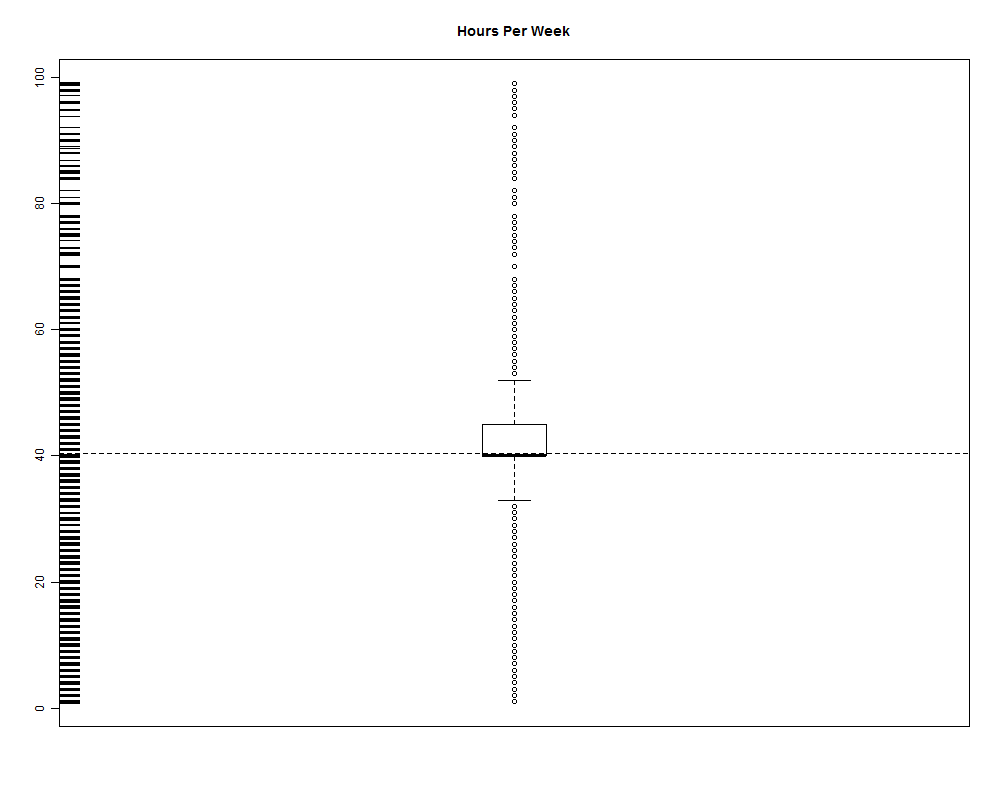
\includegraphics[width=9cm]{boxplot_hours_per_week.png}
\caption{Boxplot of the hours per week variable}
\label{fig:box_hours}
\end{figure}

\begin{figure}
\centering
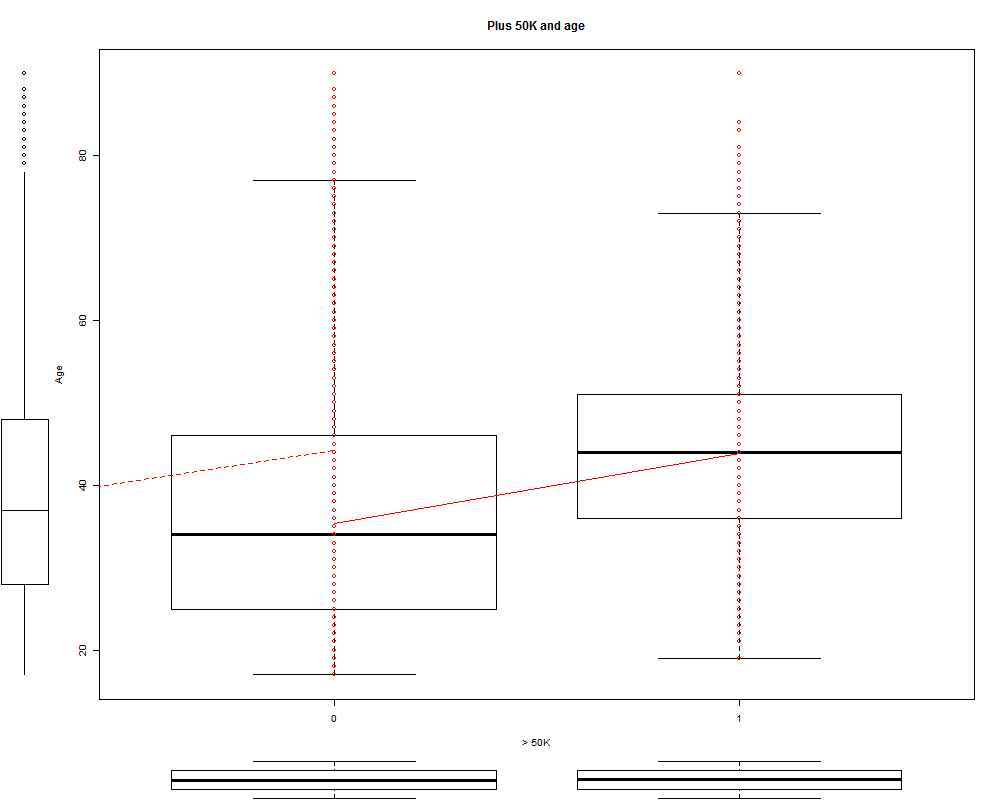
\includegraphics[width=8cm]{plot_plus_50_age.png}
\caption{Boxplot of the individuals' age, for each class of gain}
\label{fig:age_plus50}
\end{figure}

\begin{figure}
\centering
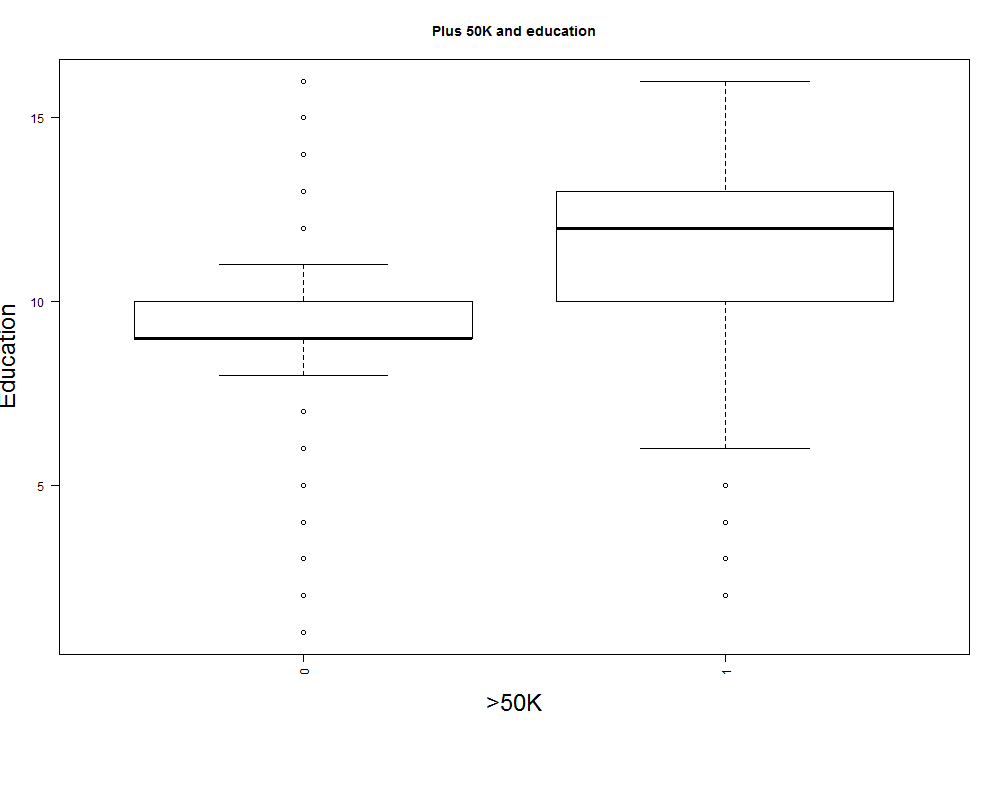
\includegraphics[width=9cm]{plot_plus_50_education_num.png}
\caption{Boxplot of the individuals' education level, for each class of gain}
\label{fig:education_plus50}
\end{figure}

\begin{figure}
\centering
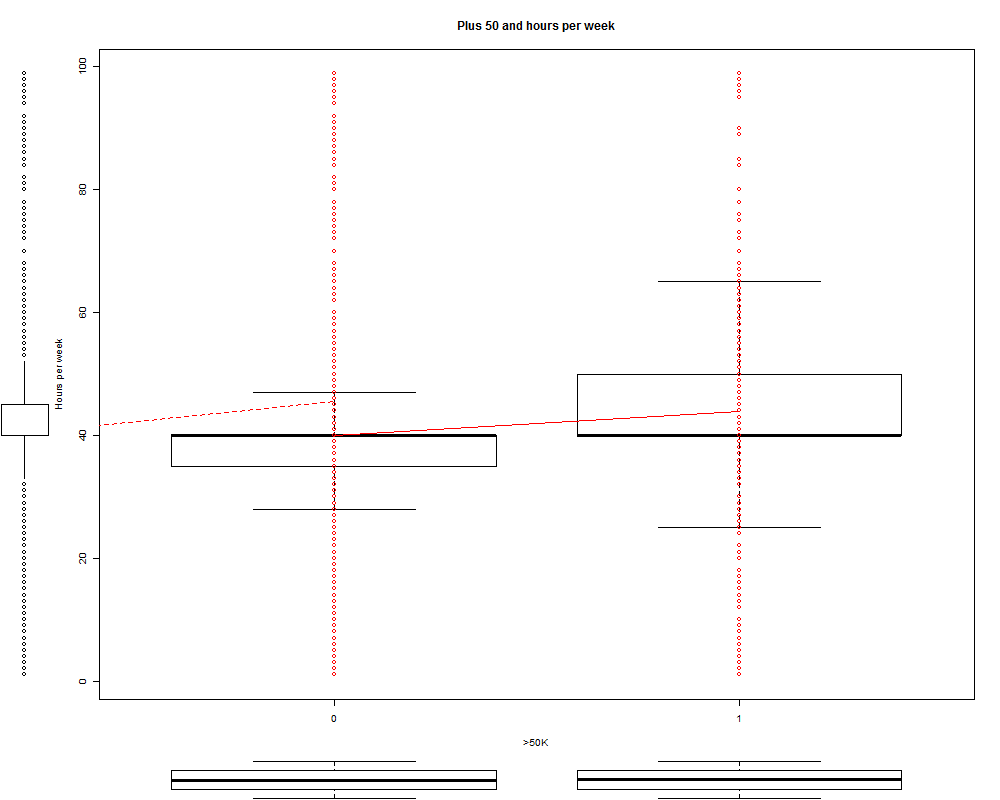
\includegraphics[width=9cm]{plot_plus_50_hpw.png}
\caption{Boxplot of the individuals' hours of work per week, for each class of 
gain}
\label{fig:hpw_plus50}
\end{figure}

\begin{figure}
\centering
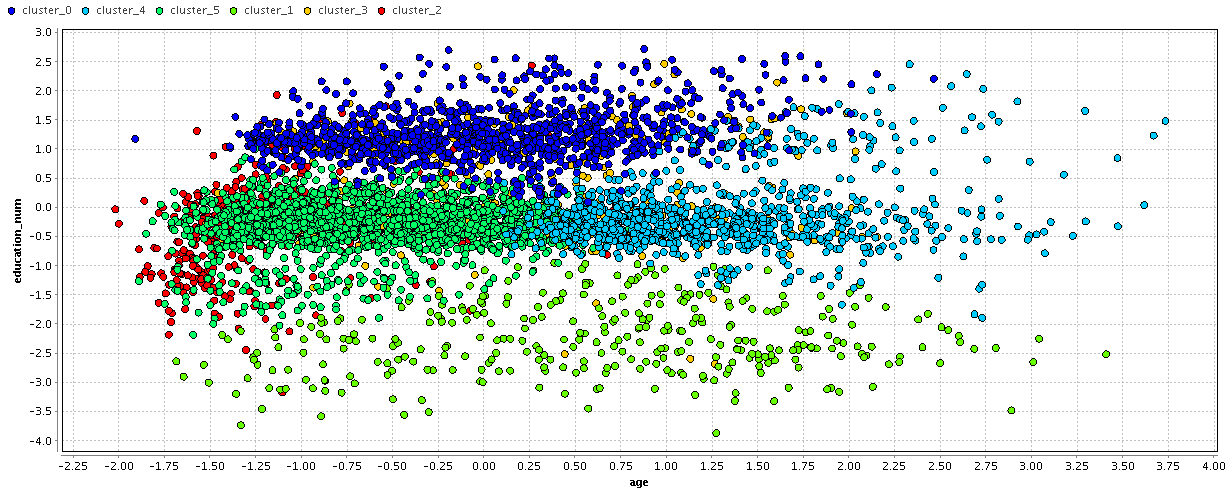
\includegraphics[width=10cm]{cluster_1_age_education.png}
\caption{Scatter plot of age and education}
\label{fig:cluster_1_age_education}
\end{figure}

\begin{figure}
\centering
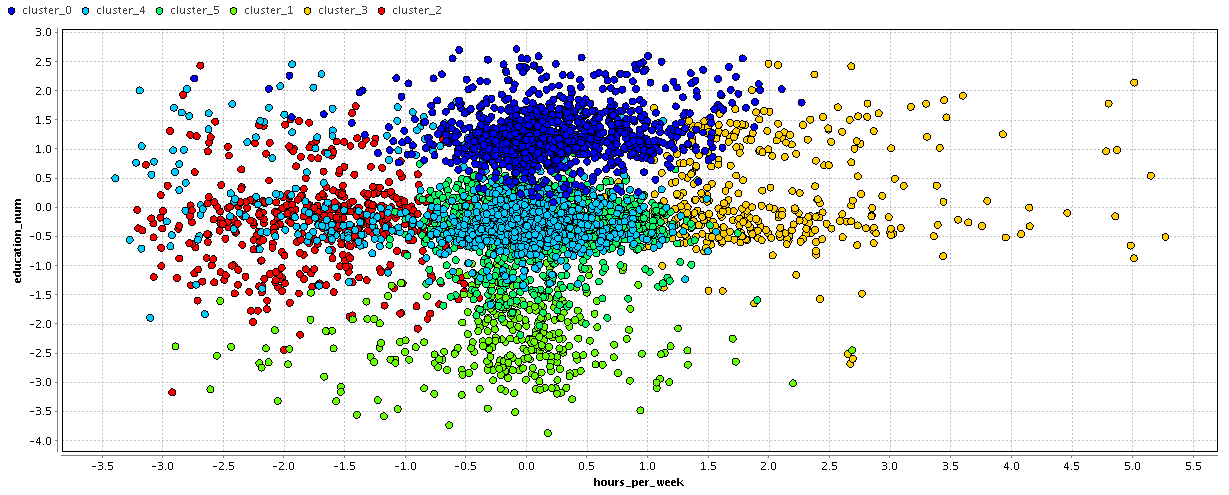
\includegraphics[width=10cm]{cluster_1_education_hpw.png}
\caption{Scatter plot of education and hours of work per week}
\label{fig:cluster_1_education_hpw}
\end{figure}

\begin{figure}
\centering
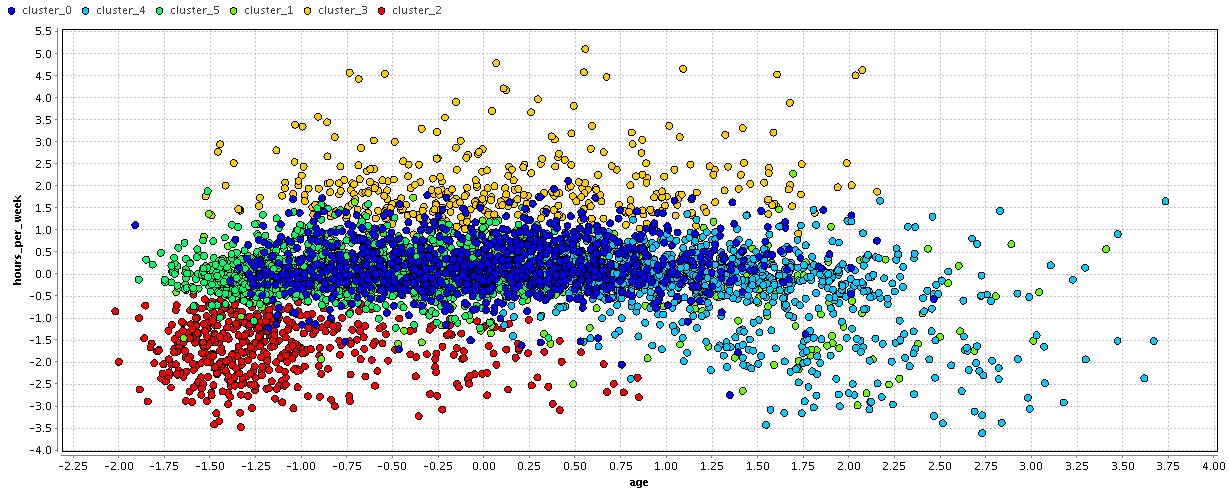
\includegraphics[width=10cm]{cluster_1_age_hpw.png}
\caption{Scatter plot of age and hours of work per week}
\label{fig:cluster_1_age_hpw}
\end{figure}

\begin{figure}
\centering
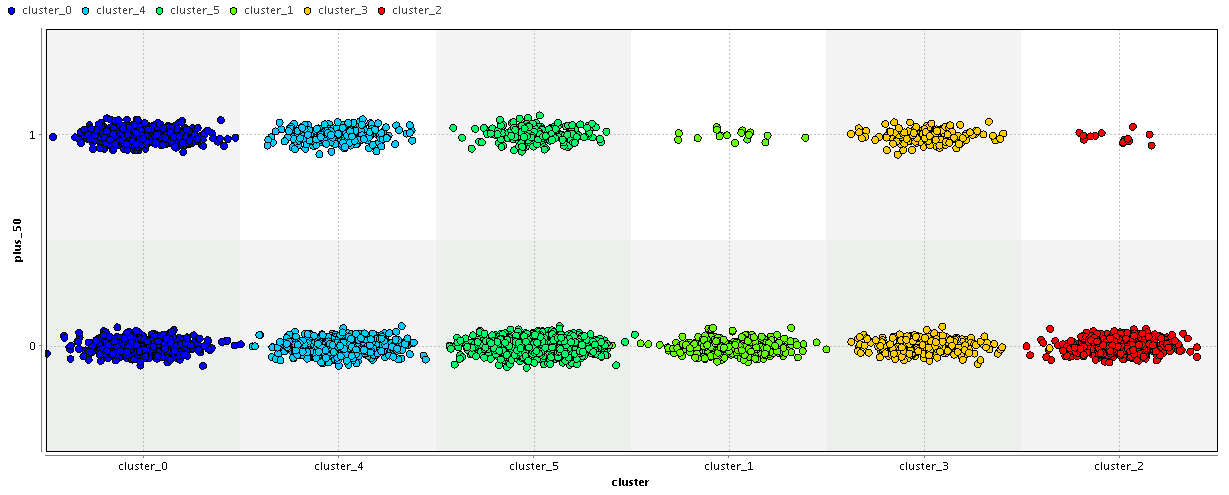
\includegraphics[width=10cm]{cluster_1_cluster_plus50.png}
\caption{Scatter plot of cluster and class values of amount gained}
\label{fig:cluster_1_cluster_plus50}
\end{figure}

\begin{figure}
\centering
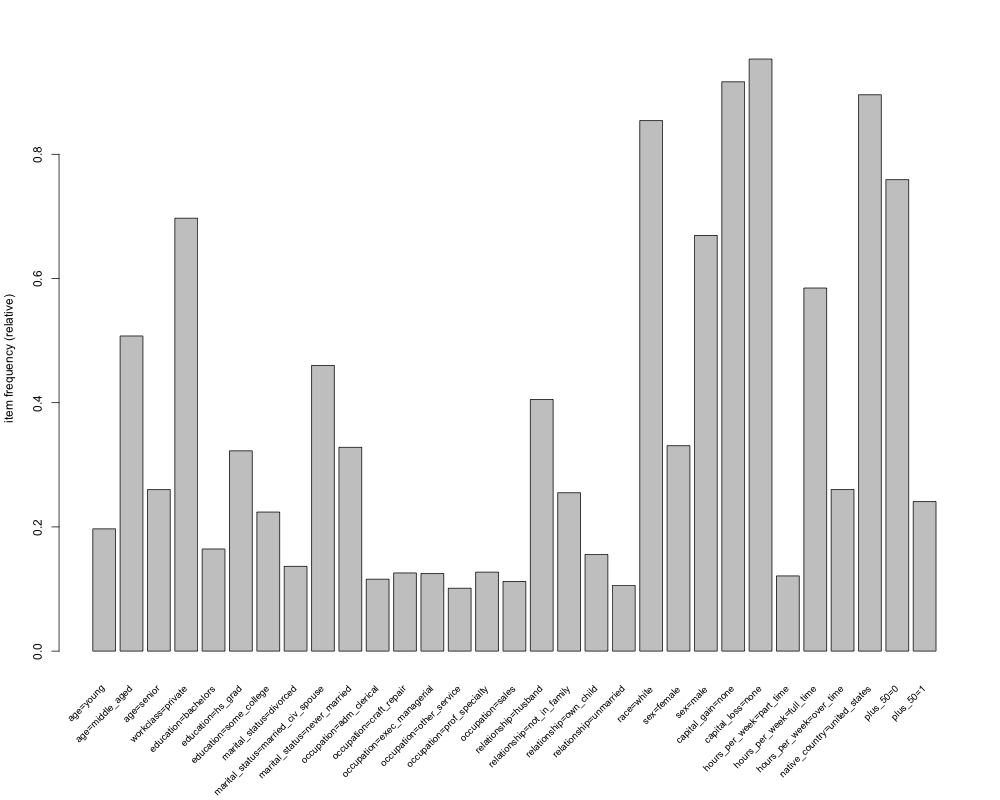
\includegraphics[width=20cm,angle=90]{item_frequency.png}
\caption{Item frequencies of items with at least 10\% support.}
\label{fig:arules_item_frequency}
\end{figure}

\clearpage
\section{Association rules}

\begin{lstlisting}[language=r,frame=single,breaklines=true,basicstyle=\footnotesize\ttfamily,caption={Association rules for small income.},label=arules_small_income]
  lhs                               rhs            support confidence     lift
1 {age=young,                                                                 
   hours_per_week=part_time}     => {plus_50=0} 0.05730782          1 1.317193
2 {age=young,                                                                 
   occupation=unknown,                                                        
   capital_gain=none}            => {plus_50=0} 0.02002396          1 1.317193
3 {age=young,                                                                 
   relationship=own_child,                                                    
   hours_per_week=part_time}     => {plus_50=0} 0.04404042          1 1.317193
4 {education=some_college,                                                    
   relationship=own_child,                                                    
   hours_per_week=part_time}     => {plus_50=0} 0.02069961          1 1.317193
5 {marital_status=never_married,                                              
   relationship=own_child,                                                    
   hours_per_week=part_time}     => {plus_50=0} 0.04689659          1 1.317193
\end{lstlisting}

\begin{lstlisting}[language=r,frame=single,breaklines=true,basicstyle=\footnotesize\ttfamily,caption={Association rules for large income.},label=arules_large_income]
  lhs                                    rhs            support confidence     lift
1 {relationship=husband,                                                           
   race=white,                                                                     
   capital_gain=high}                 => {plus_50=1} 0.02063819  0.9926145 4.121990
2 {marital_status=married_civ_spouse,                                              
   relationship=husband,                                                           
   race=white,                                                                     
   capital_gain=high}                 => {plus_50=1} 0.02063819  0.9926145 4.121990
3 {relationship=husband,                                                           
   race=white,                                                                     
   sex=male,                                                                       
   capital_gain=high}                 => {plus_50=1} 0.02063819  0.9926145 4.121990
4 {relationship=husband,                                                           
   race=white,                                                                     
   capital_gain=high,                                                              
   capital_loss=none}                 => {plus_50=1} 0.02063819  0.9926145 4.121990
5 {relationship=husband,                                                           
   capital_gain=high}                 => {plus_50=1} 0.02251159  0.9918809 4.118943
\end{lstlisting}


\clearpage
\section{Decision trees}

\begin{lstlisting}[language=c,frame=single,breaklines=true,basicstyle=\footnotesize\ttfamily,caption={Decision tree built by C4.5 with -C 0.05},label=decision_tree_c45]
capital_gain = none
|   marital_status = never_married: <50K (10228.0/340.0)
|   marital_status = married_civ_spouse
|   |   education = bachelors
|   |   |   capital_loss = none
|   |   |   |   age = young: <50K (33.0/4.0)
|   |   |   |   age = middle_aged: >50K (1287.0/515.0)
|   |   |   |   age = senior: >50K (707.0/243.0)
|   |   |   |   age = old: <50K (77.0/25.0)
|   |   |   capital_loss = low: >50K (0.0)
|   |   |   capital_loss = medium: >50K (222.0/26.0)
|   |   education = hs_grad
|   |   |   capital_loss = none: <50K (4167.0/1130.0)
|   |   |   capital_loss = low: <50K (1.0)
|   |   |   capital_loss = medium: >50K (235.0/105.0)
|   |   education = 11th: <50K (328.0/29.0)
|   |   education = masters: >50K (823.0/214.0)
|   |   education = 9th: <50K (212.0/18.0)
|   |   education = some_college: <50K (2508.0/1000.0)
|   |   education = assoc_acdm: <50K (412.0/186.0)
|   |   education = assoc_voc: <50K (596.0/251.0)
|   |   education = 7th_8th: <50K (325.0/29.0)
|   |   education = doctorate: >50K (230.0/42.0)
|   |   education = prof_school: >50K (295.0/62.0)
|   |   education = 5th_6th: <50K (161.0/11.0)
|   |   education = 10th
|   |   |   capital_loss = none: <50K (314.0/41.0)
|   |   |   capital_loss = low: <50K (0.0)
|   |   |   capital_loss = medium: >50K (9.0/2.0)
|   |   education = 1st_4th: <50K (78.0/5.0)
|   |   education = preschool: <50K (18.0)
|   |   education = 12th: <50K (119.0/21.0)
|   marital_status = divorced: <50K (4155.0/333.0)
|   marital_status = married_spouse_absent: <50K (397.0/25.0)
|   marital_status = separated: <50K (973.0/46.0)
|   marital_status = married_af_spouse
|   |   hours_per_week = part_time: <50K (2.0)
|   |   hours_per_week = full_time: <50K (3.0)
|   |   hours_per_week = over_time: >50K (13.0/4.0)
|   |   hours_per_week = workaholic: <50K (3.0)
|   marital_status = widowed: <50K (918.0/62.0)
capital_gain = low: <50K (55.0)
capital_gain = medium: <50K (1009.0/181.0)
capital_gain = high: >50K (878.0/138.0)
capital_gain = very_high: >50K (770.0/14.0)
\end{lstlisting}

\clearpage
\section{Classification Rules}
\begin{lstlisting}[language=c,frame=single,breaklines=true,basicstyle=\footnotesize\ttfamily,caption={Subset of the ordered set of rules induced by CN2 with the laplacian error estimation method},label=cn2_rules]
IF    age < 20.50
  AND capital_gain < 9720.00
  AND hours_per_week < 59.00
THEN  class = less_or_equal_than_50K  [0 2366]
ELSE
IF    19.50 < age < 21.50
  AND marital_status = never_married
  AND capital_gain < 67047.00
THEN  class = less_or_equal_than_50K  [0 664]
ELSE
IF    age < 54.50
  AND capital_gain > 10585.50
  AND hours_per_week > 33.00
THEN  class = more_than_50K  [520 0]
ELSE
IF    age < 23.50
  AND hours_per_week < 31.00
THEN  class = less_or_equal_than_50K  [0 492]
ELSE
IF    age < 24.50
  AND workclass = private
  AND relationship = own_child
  AND capital_loss < 2129.50
  AND hours_per_week > 32.50
  AND native_country = united_states
THEN  class = less_or_equal_than_50K  [0 562]
ELSE
IF    age < 60.50
  AND 7565.50 < capital_gain < 30961.50
THEN  class = more_than_50K  [445 0]
ELSE
IF    relationship = own_child
  AND race = black
  AND hours_per_week < 49.00
THEN  class = less_or_equal_than_50K  [0 261]
ELSE
IF    age < 38.50
  AND education = hs_grad
  AND marital_status = never_married
  AND relationship = own_child
  AND hours_per_week < 75.00
THEN  class = less_or_equal_than_50K  [0 378]
ELSE
IF    20.50 < age < 23.50
  AND workclass = private
  AND marital_status = never_married
  AND capital_loss < 2116.00
  AND hours_per_week > 32.50
THEN  class = less_or_equal_than_50K  [0 434]
\end{lstlisting}
\clearpage

\begin{lstlisting}[language=c,frame=single,breaklines=true,basicstyle=\footnotesize\ttfamily,caption={Subset of the prolog clauses produced by Aleph},label=ilp_clauses]
more_than_50K(A) :-
   middle_aged(A), very_high_capital_gain(A), is_native_of_united_states(A).
more_than_50K(A) :-
   education_prof_school(A), wife(A), workaholic(A).
more_than_50K(A) :-
   senior(A), work_private(A), very_high_capital_gain(A).
more_than_50K(A) :-
   senior(A), work_federal_gov(A), education_doctorate(A).
more_than_50K(A) :-
   education_doctorate(A), medium_capital_loss(A), workaholic(A).
more_than_50K(A) :-
   work_self_emp_inc(A), high_capital_gain(A), full_time_worker(A).
more_than_50K(A) :-
   middle_aged(A), education_masters(A), is_native_of_iran(A).
more_than_50K(A) :-
   senior(A), very_high_capital_gain(A), over_time_worker(A).
more_than_50K(A) :-
   other_relative(A), high_capital_gain(A).
more_than_50K(A) :-
   education_bachelors(A), occupation_other_service(A), high_capital_gain(A).
more_than_50K(A) :-
   senior(A), married_civ_spouse(A), very_high_capital_gain(A).
more_than_50K(A) :-
   senior(A), full_time_worker(A), is_native_of_cambodia(A).
more_than_50K(A) :-
   middle_aged(A), married_civ_spouse(A), is_native_of_thailand(A).
more_than_50K(A) :-
   young(A), high_capital_gain(A), over_time_worker(A).
more_than_50K(A) :-
   middle_aged(A), asian_pac_islander(A), high_capital_gain(A).
more_than_50K(A) :-
   occupation_protective_serv(A), high_capital_gain(A), full_time_worker(A).
more_than_50K(A) :-
   work_state_gov(A), occupation_exec_managerial(A), high_capital_gain(A).
more_than_50K(A) :-
   education_bachelors(A), occupation_tech_support(A), wife(A).
more_than_50K(A) :-
   education_prof_school(A), very_high_capital_gain(A).
more_than_50K(A) :-
   high_capital_gain(A), full_time_worker(A), is_native_of_canada(A).
more_than_50K(A) :-
   education_prof_school(A), medium_capital_loss(A), over_time_worker(A).
more_than_50K(A) :-
   work_private(A), education_doctorate(A), is_native_of_taiwan(A).
\end{lstlisting}


\end{document}
